\chapter{Random vectors and the Gaussian}\label{ch02}
\providecommand{\Kc}{K_c}
% Short running heads for long sentence-style section titles. The original
% \sectionmark is saved here and restored at the end of the chapter.
\let\ompSavedSectionmark\sectionmark
\providecommand{\ompnexthead}[1]{\def\ompheadtext{#1}%
  \renewcommand{\sectionmark}[1]{\markright{\MakeUppercase{\thesection.\ \ompheadtext}}}}

Primer~S of \emph{Data Mining as Observation} treats one random variable at a
time, and two at most through a covariance and a correlation. The programme
works with random \emph{vectors}. A source is a vector, a reconstruction error
is a vector, and a consumer reads a vector through a matrix. This chapter
builds the vector versions of mean and variance, then the one distribution the
programme assumes whenever it wants a closed form, the multivariate normal.

Three ideas carry the chapter. A linear map moves a covariance by
$\Sigma\mapsto A\Sigma A\T$. Conditioning a Gaussian on part of itself leaves
a Schur complement, the matrix of chapter~1's section on block elimination.
And the best estimate of a vector, under any quadratic loss a consumer might
impose, is the conditional mean. The Kalman filter, the Cram\'er--Rao bound and
the Gaussian mutual information all follow from those three. Every number in
the worked examples is recomputed by \texttt{checks/ch02\_examples.py}.

% ---------------------------------------------------------------------------
\ompnexthead{Mean vectors and covariance matrices}
\section{A linear map moves a mean by \texorpdfstring{$A\mu$}{A mu} and a covariance by \texorpdfstring{$A\Sigma A\T$}{A Sigma A transpose}}\label{sec:ch02:moments}

A random vector $x\in\R^d$ is a list of $d$ random variables observed
together. Its mean is the list of their means, and its covariance matrix
collects every variance and every covariance of Primer~S, section~S.5, into
one symmetric table.

\begin{definition}[Mean vector, covariance and cross-covariance]\label{def:ch02:cov}
\begin{equation}\label{eq:ch02:cov}
\mu=\E[x],\qquad
\Sigma=\Cov(x)=\E\big[(x-\mu)(x-\mu)\T\big]=\E[xx\T]-\mu\mu\T,\qquad
\Cov(x,y)=\E\big[(x-\mu_x)(y-\mu_y)\T\big].
\end{equation}
\end{definition}

The diagonal entries of $\Sigma$ are the variances $\Var(x_i)$, and the
off-diagonal entries are the covariances $\Cov(x_i,x_j)$. The matrix is
symmetric. It is also positive semidefinite, because for any fixed vector $u$
the number $u\T\Sigma u=\E[(u\T(x-\mu))^2]$ is the variance of the scalar
$u\T x$ and cannot be negative. The covariance is singular exactly when some
nonzero combination $u\T x$ is constant, that is, when the vector lives on a
lower-dimensional flat. The cross-covariance $\Cov(x,y)$ of two vectors of
lengths $d$ and $p$ is a $d\times p$ matrix and need not be square or symmetric,
and $\Cov(y,x)=\Cov(x,y)\T$.

Linearity of expectation gives the rule that the whole chapter runs on. For a
fixed matrix $A$, a fixed matrix $B$ and a fixed vector $b$,
\begin{equation}\label{eq:ch02:linmap}
\E[Ax+b]=A\mu+b,\qquad \Cov(Ax+b)=A\Sigma A\T,\qquad \Cov(Ax,Bx)=A\Sigma B\T .
\end{equation}
The proof is one line, $Ax+b-(A\mu+b)=A(x-\mu)$, so the outer product is
$A(x-\mu)(x-\mu)\T A\T$, and the expectation passes through the fixed
matrices. Three special cases recur. With $A=u\T$ a row, the variance of a
single read is $u\T\Sigma u$, equation~0.4 of chapter~0. With $A=\Sigma^{-1/2}$
the covariance becomes $I$, which is whitening (chapter~1). With $A$ a
consumer's Jacobian $J$, the covariance of the consumer's output error is
$J\Sd J\T$ to first order, and the output metric $G$ turns it into the scalar
$\tr(GJ\Sd J\T)=\tr(J\T GJ\,\Sd)=\tr(\PC\Sd)$. That is where the read operator
of chapter~0 comes from.

For independent vectors the covariances add, $\Cov(x+v)=\Cov(x)+\Cov(v)$, since
the cross terms $\Cov(x,v)$ vanish. Uncorrelated is enough for this. A sensor
reading $y=Hx+v$ with noise $v$ uncorrelated with $x$ therefore has
\begin{equation}\label{eq:ch02:sensor}
\Cov(y)=H\Sigma_xH\T+R,\qquad \Cov(x,y)=\Sigma_xH\T,\qquad R=\Cov(v).
\end{equation}
These two matrices are all the later sections need to estimate $x$ from $y$.

\begin{example}[A sum and a difference]\label{ex:ch02:linmap}
Let $x$ have mean $\mu=(1,2)\T$ and covariance
$\Sigma=\begin{pmatrix}2&1\\1&3\end{pmatrix}$, and let
$A=\begin{pmatrix}1&1\\1&-1\end{pmatrix}$, so $Ax$ lists the sum and the
difference. Then $A\mu=(3,-1)\T$ and
\[
A\Sigma=\begin{pmatrix}3&4\\1&-2\end{pmatrix},\qquad
A\Sigma A\T=\begin{pmatrix}7&-1\\-1&3\end{pmatrix}.
\]
Directly, $\Var(x_1+x_2)=2+3+2\cdot1=7$, $\Var(x_1-x_2)=2+3-2=3$ and
$\Cov(x_1+x_2,\,x_1-x_2)=\Var(x_1)-\Var(x_2)=2-3=-1$. The sum and difference
are correlated even though $A$ has orthogonal rows, because the two
coordinates have different variances.
\end{example}

\buildson{Primer~S, sections~S.2 and S.5. Chapter~0 of \emph{Data Mining as
Observation}, section~0.3. Chapter~1, the trace identities.}
\usedin{Every later section. Chapter~3, where differential entropy depends on
$\Sigma$ through $\det\Sigma$. Chapter~6, where $\PC=J\T GJ$.}

% ---------------------------------------------------------------------------
\ompnexthead{The multivariate normal}
\section{The multivariate normal is fixed by its mean and covariance, and its level sets are ellipsoids}\label{sec:ch02:gauss}

The normal distribution of Primer~S, section~S.3, has a vector version with
one parameter for every mean and every covariance.

\begin{definition}[Multivariate normal]\label{def:ch02:mvn}
A random vector $x\in\R^d$ is \emph{normal}, written $x\sim\Normal(\mu,\Sigma)$,
when it equals $\mu+\Sigma^{1/2}z$ with $z$ a vector of $d$ independent
standard normals. For $\Sigma\pd0$ its density is
\begin{equation}\label{eq:ch02:mvn}
p(x)=\frac{1}{(2\pi)^{d/2}\det(\Sigma)^{1/2}}\exp\!\Big(-\tfrac12(x-\mu)\T\Sigma^{-1}(x-\mu)\Big).
\end{equation}
\end{definition}

The density follows from the change of variables $x=\mu+\Sigma^{1/2}z$. The
density of $z$ is a product of $d$ scalar normals,
$(2\pi)^{-d/2}\exp(-\tfrac12z\T z)$. Substituting
$z=\Sigma^{-1/2}(x-\mu)$ gives the quadratic form in the exponent, and the
Jacobian of the substitution contributes $\det(\Sigma^{-1/2})=\det(\Sigma)^{-1/2}$.

The exponent is $-\tfrac12$ times the squared \emph{Mahalanobis distance}
\begin{equation}\label{eq:ch02:mahal}
r^2(x)=(x-\mu)\T\Sigma^{-1}(x-\mu)=\norm{\Sigma^{-1/2}(x-\mu)}^2 ,
\end{equation}
the squared Euclidean length after whitening. The density is constant where
$r$ is constant, so the level sets are the ellipsoids $r^2=c$. Writing
$\Sigma=\sum_i\lambda_iv_iv_i\T$, the ellipsoid $r^2=c$ has its axes along the
eigenvectors $v_i$, with semi-axis lengths $\sqrt{c\lambda_i}$. Since $r^2$ is
a sum of $d$ squared independent standard normals, it has the chi-square
distribution with $d$ degrees of freedom. In two dimensions that distribution
is exponential with mean $2$, so
\begin{equation}\label{eq:ch02:chi2}
\Pr\big[r^2\le c\big]=1-e^{-c/2}\qquad(d=2).
\end{equation}

Two properties make the Gaussian the programme's default closed-form source.
First, an affine map of a Gaussian is Gaussian, with the moments of
\cref{eq:ch02:linmap}, because $Ax+b=(A\mu+b)+A\Sigma^{1/2}z$ is again an
affine function of $z$. Every marginal is therefore Gaussian, with the
matching sub-vector of $\mu$ and sub-block of $\Sigma$. Second, for
\emph{jointly} Gaussian vectors, uncorrelated means independent. If
$\Cov(x,y)=0$, the joint covariance is block diagonal, the quadratic form in
\cref{eq:ch02:mvn} splits into an $x$ part and a $y$ part, and the density
factors. The word ``jointly'' carries the weight. Two variables can each be
normal and uncorrelated without being independent (\cref{exr:ch02:notjoint}).

\begin{example}[Ellipses of a correlated pair]\label{ex:ch02:mvn}
Let $\mu=0$ and $\Sigma=\begin{pmatrix}5&2\\2&2\end{pmatrix}$, the matrix of
chapter~1's spectral example, with eigenvalues $6$ and $1$ along
$(2,1)\T/\sqrt5$ and $(1,-2)\T/\sqrt5$. Its determinant is $6$ and
\[
\Sigma^{-1}=\tfrac16\begin{pmatrix}2&-2\\-2&5\end{pmatrix}.
\]
The density at the mean is $1/(2\pi\sqrt6)\approx0.06497$. At $x=(1,1)\T$ the
Mahalanobis form is $(2-2-2+5)/6=\tfrac12$, so the density there is
$e^{-1/4}/(2\pi\sqrt6)\approx0.0506$, and by \cref{eq:ch02:chi2} the
probability of falling inside that point's ellipse is $1-e^{-1/4}\approx0.2212$.
The ellipse containing probability $0.95$ has $c=-2\log0.05\approx5.991$, so
its semi-axes are $\sqrt{6\cdot5.991}\approx5.996$ along $(2,1)\T$ and
$\sqrt{5.991}\approx2.448$ along $(1,-2)\T$. \Cref{fig:ch02:ellipse} draws both
levels. The point $(1,1)\T$ is at Euclidean distance $\sqrt2$ from the mean, and
the point $(1,-2)\T/\sqrt5\cdot\sqrt2$ along the thin axis is at the same
Euclidean distance, but its Mahalanobis form is $2$, four times larger. Distance
in a Gaussian is measured in units of the spread along each direction.
\end{example}

\begin{figure}[t]
\centering
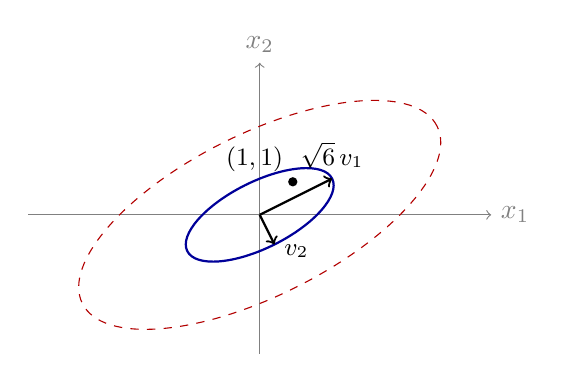
\begin{tikzpicture}[scale=0.42]
\draw[->,gray] (-7,0)--(7,0) node[right] {$x_1$};
\draw[->,gray] (0,-4.2)--(0,4.6) node[above] {$x_2$};
\draw[thick,blue!60!black,rotate=26.565] (0,0) ellipse (2.449 and 1);
\draw[dashed,red!70!black,rotate=26.565] (0,0) ellipse (5.996 and 2.448);
\draw[->,thick,rotate=26.565] (0,0)--(2.449,0) node[above,pos=1] {\small $\sqrt6\,v_1$};
\draw[->,thick,rotate=26.565] (0,0)--(0,-1);
\node[right] at (0.45,-1.1) {\small $v_2$};
\fill (1,1) circle (4pt) node[above left] {\small $(1,1)$};
\end{tikzpicture}
\caption{Level sets of $\Normal(0,\Sigma)$ with $\Sigma$ having rows $(5,2)$ and
$(2,2)$. The solid ellipse is $r^2=1$, with semi-axes $\sqrt6$ and $1$ along the
eigenvectors. The dashed ellipse is $r^2\approx5.991$ and contains probability
$0.95$. The marked point has $r^2=\tfrac12$.}
\label{fig:ch02:ellipse}
\end{figure}

\inproject{\nolinkurl{geometric-observation/paper/observation-theory.tex} assumes a
Gaussian source whenever it states a closed form. The appendix ``The price of a
misidentified observer'' opens with ``Throughout $X\sim\mathcal N(0,\Sigma_x)$,
$\Sigma_x\succ0$'', and the two-stage rate region of section ``Successive
refinement across observers'' is stated for a Gaussian source. The discussion
section lists non-Gaussian sources as open.}

\buildson{Primer~S, section~S.3. Chapter~1, whitening and the spectral theorem.}
\usedin{\Cref{sec:ch02:cond,sec:ch02:mi}. Chapter~3, differential entropy of a
Gaussian. Chapter~7, the Gaussian model behind scalar quantizer codebooks.}

% ---------------------------------------------------------------------------
\ompnexthead{Gaussian conditioning}
\section{Conditioning a Gaussian on part of itself leaves a Schur complement}\label{sec:ch02:cond}

Split a jointly Gaussian vector into a part $x$ we want and a part $y$ we
observe. The question is what the distribution of $x$ becomes once $y$ is
known. The answer is Gaussian again, with a mean that moves linearly with $y$
and a covariance that does not depend on $y$ at all.

\begin{theorem}[Gaussian conditioning]\label{thm:ch02:cond}
Let
\[
\begin{pmatrix}x\\y\end{pmatrix}\sim\Normal\!\left(\begin{pmatrix}\mu_x\\\mu_y\end{pmatrix},
\begin{pmatrix}\Sigma_{xx}&\Sigma_{xy}\\\Sigma_{yx}&\Sigma_{yy}\end{pmatrix}\right),\qquad \Sigma_{yy}\pd0 .
\]
Then $x\mid y\sim\Normal\big(\mu_{x\mid y},\Sigma_{x\mid y}\big)$ with
\begin{equation}\label{eq:ch02:cond}
\mu_{x\mid y}=\mu_x+K(y-\mu_y),\qquad
\Sigma_{x\mid y}=\Sigma_{xx}-\Sigma_{xy}\Sigma_{yy}^{-1}\Sigma_{yx},\qquad
K=\Sigma_{xy}\Sigma_{yy}^{-1}.
\end{equation}
\end{theorem}

\begin{proof}
Define the residual $e=x-\mu_x-K(y-\mu_y)$. It is an affine function of the
joint vector, so $(e,y)$ is jointly Gaussian. By \cref{eq:ch02:linmap} its
cross-covariance with $y$ is
$\Cov(e,y)=\Sigma_{xy}-K\Sigma_{yy}=\Sigma_{xy}-\Sigma_{xy}=0$. Jointly Gaussian
and uncorrelated means independent, so $e$ is independent of $y$, with mean $0$
and covariance
\[
\Cov(e)=\Sigma_{xx}-K\Sigma_{yx}-\Sigma_{xy}K\T+K\Sigma_{yy}K\T
=\Sigma_{xx}-\Sigma_{xy}\Sigma_{yy}^{-1}\Sigma_{yx}.
\]
Now $x=\mu_x+K(y-\mu_y)+e$. Given $y$, the first two terms are fixed and $e$
keeps its own distribution because it is independent of $y$. That is the claim.
\end{proof}

The conditional covariance is the Schur complement of $\Sigma_{yy}$ in the
joint covariance, chapter~1's matrix $D-B\T A^{-1}B$ with the blocks renamed.
Three consequences are worth stating. First, by the Schur complement test it
is PSD and it satisfies $\Sigma_{x\mid y}\preceq\Sigma_{xx}$, since the
subtracted term $\Sigma_{xy}\Sigma_{yy}^{-1}\Sigma_{yx}$ is PSD. Observing
never increases uncertainty in the Loewner order, which by chapter~1's
every-reader characterization means it never increases any consumer's
weighted error. Second, $\Sigma_{x\mid y}$ does not involve the observed value
of $y$. How much is learned is fixed in advance by the joint covariance, and
only where the estimate lands depends on the data. This is special to the
Gaussian. Third, by the block inverse of chapter~1, the $xx$ block of the
joint \emph{precision} matrix $\Sigma^{-1}$ is $\Sigma_{x\mid y}^{-1}$.
Conditional covariances can be read off the inverse of the joint covariance
without any further algebra,
\begin{equation}\label{eq:ch02:precision}
\big(\Sigma^{-1}\big)_{xx}=\Sigma_{x\mid y}^{-1}.
\end{equation}

\begin{example}[Scalar and vector conditioning]\label{ex:ch02:cond}
Let $(x,y)$ be zero-mean Gaussian with $\Var x=4$, $\Var y=2$ and
$\Cov(x,y)=2$. Then $K=2/2=1$ and $\Sigma_{x\mid y}=4-2\cdot2/2=2$. Observing
$y=1.5$ gives $x\mid y\sim\Normal(1.5,2)$. Half the variance of $x$ is
removed, and it would be removed whatever value $y$ took.

For a vector observation, use chapter~1's three-by-three matrix as a joint
covariance, with $x$ the first coordinate and $y$ the last two,
\[
\Sigma=\begin{pmatrix}4&2&2\\2&2&1\\2&1&3\end{pmatrix},\qquad
\Sigma_{xy}=(2,2),\qquad
\Sigma_{yy}^{-1}=\tfrac15\begin{pmatrix}3&-1\\-1&2\end{pmatrix}.
\]
Then $K=(2,2)\Sigma_{yy}^{-1}=\tfrac15(4,2)=(0.8,0.4)$ and
$\Sigma_{x\mid y}=4-(0.8\cdot2+0.4\cdot2)=1.6$. By \cref{eq:ch02:precision}
this should be $1/(\Sigma^{-1})_{11}$. The cofactor of the $(1,1)$ entry is
$\det\Sigma_{yy}=5$ and $\det\Sigma=8$, so $(\Sigma^{-1})_{11}=\tfrac58=0.625$
and $1/0.625=1.6$. With zero means and an observed $y=(1,2)\T$, the conditional
mean is $0.8\cdot1+0.4\cdot2=1.6$.

Conditioning the other way, on $x$, leaves the Schur complement of the
$(1,1)$ entry, which chapter~1 computed as $\diag(1,2)$. So given $x$, the
last two coordinates are uncorrelated, with variances $1$ and $2$ and
conditional mean $\tfrac24x\,(1,1)\T=\tfrac{x}{2}(1,1)\T$.
\end{example}

\buildson{Chapter~1, the Schur complement and the block inverse.
\Cref{sec:ch02:moments,sec:ch02:gauss}.}
\usedin{\Cref{sec:ch02:mmse,sec:ch02:kalman,sec:ch02:mi}. Chapter~3, conditional
entropy. Chapter~6, side information and leakage.}

% ---------------------------------------------------------------------------
\ompnexthead{MMSE and LMMSE estimation}
\section{The conditional mean is the best estimate for every quadratic loss, and the linear estimate needs only second moments}\label{sec:ch02:mmse}

An estimator is any function $\hat x=g(y)$ of the data. A consumer scores its
error through a PSD weight $P$, and the expected loss is
$\E[(x-\hat x)\T P(x-\hat x)]$. The surprising fact is that one estimator
minimizes this loss for every $P$ at once.

\begin{theorem}[The conditional mean is optimal for every reader]\label{thm:ch02:mmse}
Let $m(y)=\E[x\mid y]$ and $\Sigma_{x\mid y}=\Cov(x\mid y)$. For every
estimator $g$ and every $P\psd0$,
\begin{equation}\label{eq:ch02:mmse}
\E\big[(x-g)\T P(x-g)\mid y\big]
=\tr\big(P\,\Sigma_{x\mid y}\big)+(m-g)\T P\,(m-g)\ \ge\ \tr\big(P\,\Sigma_{x\mid y}\big).
\end{equation}
\end{theorem}

\begin{proof}
Write $x-g=(x-m)+(m-g)$. Given $y$, the second part is fixed and the first has
conditional mean zero, so the cross term vanishes. The first part contributes
$\E[(x-m)\T P(x-m)\mid y]=\tr(P\,\Sigma_{x\mid y})$ by the trace identity of
chapter~1, and the second contributes $(m-g)\T P(m-g)\ge0$.
\end{proof}

The conditional mean is the minimum mean squared error (MMSE) estimator, and
the theorem shows that changing the reader's weight $P$ does not change it. A
consumer cannot improve on the posterior mean by asking for its own estimator.
The consumer changes the \emph{score}, $\tr(P\Sigma_{x\mid y})$, and so changes
which measurements or which descriptions are worth paying for, but not the
estimate built from a given set of them \cite{kay1993}.

The conditional mean can be hard to compute. If only the means and
covariances of $(x,y)$ are known, the best estimator among \emph{affine}
functions $\hat x=a+By$ is available in closed form. Minimizing the trace of
the error covariance over $a$ and $B$ gives the linear MMSE (LMMSE) estimator,
\begin{equation}\label{eq:ch02:lmmse}
\hat x_{\mathrm{L}}=\mu_x+K(y-\mu_y),\qquad K=\Sigma_{xy}\Sigma_{yy}^{-1},\qquad
\Cov(x-\hat x_{\mathrm{L}})=\Sigma_{xx}-\Sigma_{xy}\Sigma_{yy}^{-1}\Sigma_{yx}.
\end{equation}
The formula is the Gaussian conditional mean of \cref{eq:ch02:cond}, but its
derivation needs no Gaussian assumption. What characterizes it is the
\emph{orthogonality principle}. The error is uncorrelated with every
affine function of the data,
\begin{equation}\label{eq:ch02:orth}
\E\big[x-\hat x_{\mathrm L}\big]=0,\qquad \E\big[(x-\hat x_{\mathrm L})(y-\mu_y)\T\big]=0 .
\end{equation}
Indeed $\E[(x-\hat x_{\mathrm L})(y-\mu_y)\T]=\Sigma_{xy}-K\Sigma_{yy}=0$. If
any affine function of $y$ still correlated with the error, adding a multiple
of it to the estimate would reduce the error, so orthogonality is both
necessary and sufficient. The picture is chapter~1's projection. With the
inner product $\inner{u}{w}=\E[uw]$ on zero-mean random variables, the LMMSE
estimate is the orthogonal projection of $x$ onto the span of the data.

For jointly Gaussian $(x,y)$ the two estimators coincide. In general the LMMSE
error covariance is an upper bound on the MMSE error covariance, and the two
can be far apart. The LMMSE estimator sees only correlation, and dependence
that is not correlation is invisible to it.

\begin{example}[A noisy reading, and a dependence correlation misses]\label{ex:ch02:mmse}
Let $x\sim\Normal(0,4)$ and $y=x+v$ with $v\sim\Normal(0,1)$ independent of
$x$. By \cref{eq:ch02:sensor}, $\Sigma_{yy}=5$ and $\Sigma_{xy}=4$, so
$K=0.8$ and the error variance is $4-16/5=0.8$. The same number is
$(1/4+1/1)^{-1}=0.8$, the reciprocal of the summed precisions, a form
\cref{sec:ch02:fisher} explains. A reading of $y=2.5$ gives the estimate
$\hat x=2$, shrunk toward the prior mean $0$.

For a non-Gaussian case, let $y$ take the values $-1,0,1$ with probability
$\tfrac13$ each, and let $x=y^2$. Then $\E[x]=\tfrac23$ and
$\Cov(x,y)=\E[y^3]-\E[y^2]\E[y]=0$. The LMMSE gain is $K=0$, the LMMSE estimate
is the constant $\tfrac23$, and its mean squared error is
$\Var(x)=\tfrac23-\tfrac49=\tfrac29$. The conditional mean is $\E[x\mid y]=y^2$,
which is exact, with error $0$. Uncorrelated is not independent.
\end{example}

\inproject{\nolinkurl{geometric-observation/paper/ot-estimation-control.tex},
section ``A boundary proposition'' (label \texttt{sec:boundary}), proves
\cref{thm:ch02:mmse} as the proposition ``Weighted posterior-mean invariance'',
notes that in the linear-Gaussian case the minimizer is the Kalman estimate, and
draws the conclusion that the programme does not produce a new Kalman filter.
The remark that follows explains that a read operator depending on $x$ breaks
the invariance. In \nolinkurl{geometric-observation/paper/observation-theory.tex}
the same split appears as the lemma ``Conditional mean serves every observer''.}

\buildson{\Cref{sec:ch02:cond}. Chapter~1, the trace identity and the
orthogonal projector.}
\usedin{\Cref{sec:ch02:kalman}. Chapter~3, the converse half of Gaussian
rate--distortion. Chapter~6, the boundary between estimation and observation.}

% ---------------------------------------------------------------------------
\ompnexthead{The Kalman filter}
\section{The Kalman filter is Gaussian conditioning repeated in time}\label{sec:ch02:kalman}

A state $x_k$ evolves through a linear system and is observed through a noisy
linear sensor,
\begin{equation}\label{eq:ch02:model}
x_{k}=F x_{k-1}+w_k,\qquad y_k=Hx_k+v_k,\qquad
w_k\sim\Normal(0,Q),\quad v_k\sim\Normal(0,R),
\end{equation}
with all noises independent of each other and of the initial state
$x_0\sim\Normal(m_0,\Sigma_0)$. The Kalman filter computes the conditional
distribution of $x_k$ given the readings $y_1,\dots,y_k$ \cite{kalman1960}. Because
everything is jointly Gaussian, that distribution is Gaussian, and the filter
only has to carry its mean $m_k$ and covariance $\Sigma_k$ from one step to the
next. To keep the read operator's letter free, this book writes the filter's
covariances as $\Sigma$, not as the $P$ of many control texts.

Each step has two halves. The \emph{predict} half pushes the current belief
through the dynamics with \cref{eq:ch02:linmap}, adding the process noise,
\begin{equation}\label{eq:ch02:predict}
m_k^-=F m_{k-1},\qquad \Sigma_k^-=F\Sigma_{k-1}F\T+Q .
\end{equation}
The \emph{update} half conditions on the new reading. Under the predicted
belief, $(x_k,y_k)$ is jointly Gaussian with $\Cov(y_k)=H\Sigma_k^-H\T+R$ and
$\Cov(x_k,y_k)=\Sigma_k^-H\T$, by \cref{eq:ch02:sensor}. Plugging these blocks
into \cref{eq:ch02:cond} gives the update,
\begin{equation}\label{eq:ch02:update}
S_k=H\Sigma_k^-H\T+R,\qquad K_k=\Sigma_k^-H\T S_k^{-1},\qquad
m_k=m_k^-+K_k\big(y_k-Hm_k^-\big),\qquad
\Sigma_k=\Sigma_k^--K_kS_kK_k\T .
\end{equation}
Nothing new has been derived. The innovation $y_k-Hm_k^-$ is the surprise in
the reading, $S_k$ is its covariance, $K_k$ is the gain $\Sigma_{xy}\Sigma_{yy}^{-1}$
of \cref{eq:ch02:cond}, and $\Sigma_k$ is the Schur complement. By
\cref{thm:ch02:mmse}, $m_k$ is the best estimate for every PSD reader. Two
equivalent forms of the covariance update are in common use,
\begin{equation}\label{eq:ch02:joseph}
\Sigma_k=(I-K_kH)\Sigma_k^-
=(I-K_kH)\Sigma_k^-(I-K_kH)\T+K_kRK_k\T .
\end{equation}
The second, the Joseph form, is a sum of PSD terms, so rounding errors cannot
make it lose positive semidefiniteness. Anderson and Moore treat the filter
in full \cite{andersonmoore1979}.

As in \cref{sec:ch02:cond}, the covariances $\Sigma_k^-$ and $\Sigma_k$ never
involve the readings. They can be computed before any data arrive, and for a
time-invariant model they usually settle to a steady state.

\begin{example}[A scalar random walk]\label{ex:ch02:kalman}
Let $F=1$, $Q=1$, $H=1$ and $R=2$, with $m_0=0$ and $\Sigma_0=4$. The readings
are $y_1=2$ and $y_2=1$.

Step one. Predict $m_1^-=0$ and $\Sigma_1^-=4+1=5$. Update with $S_1=5+2=7$,
$K_1=\tfrac57$, $m_1=\tfrac57\cdot2=\tfrac{10}7\approx1.4286$ and
$\Sigma_1=5-\tfrac{25}{7}=\tfrac{10}7\approx1.4286$.

Step two. Predict $m_2^-=\tfrac{10}7$ and $\Sigma_2^-=\tfrac{10}7+1=\tfrac{17}7\approx2.4286$.
Update with $S_2=\tfrac{17}7+2=\tfrac{31}7$ and $K_2=\tfrac{17}{31}\approx0.5484$.
The innovation is $1-\tfrac{10}7=-\tfrac37$, so
$m_2=\tfrac{10}7-\tfrac{17}{31}\cdot\tfrac37=\tfrac{37}{31}\approx1.1935$ and
$\Sigma_2=\tfrac{17}7\cdot\big(1-\tfrac{17}{31}\big)=\tfrac{34}{31}\approx1.0968$.

Steady state. A fixed point has $\Sigma^-=\Sigma+1$ and
$\Sigma=\Sigma^-\cdot2/(\Sigma^-+2)$. Substituting gives
$\Sigma^2+\Sigma-2=0$, so $\Sigma=1$, $\Sigma^-=2$ and $K=\tfrac12$. The two
computed steps, $\tfrac{10}7$ and $\tfrac{34}{31}$, are approaching $1$.
\end{example}

\begin{example}[Position read, velocity learned]\label{ex:ch02:kalman2}
Track position and velocity with $F=\begin{pmatrix}1&1\\0&1\end{pmatrix}$,
process noise $Q=\diag(0,1)$ on the velocity, and a position sensor $H=(1,0)$
with $R=1$. Start from $m_0=(0,1)\T$ and $\Sigma_0=I$. The prediction is
\[
m_1^-=(1,1)\T,\qquad
\Sigma_1^-=F F\T+Q=\begin{pmatrix}2&1\\1&1\end{pmatrix}+\begin{pmatrix}0&0\\0&1\end{pmatrix}=\begin{pmatrix}2&1\\1&2\end{pmatrix}.
\]
Then $S_1=2+1=3$ and $K_1=(2,1)\T/3$. A reading $y_1=1.5$ has innovation
$0.5$, so $m_1=(1,1)\T+\tfrac{0.5}{3}(2,1)\T=(\tfrac43,\tfrac76)\T$, and
\[
\Sigma_1=\begin{pmatrix}2&1\\1&2\end{pmatrix}-\tfrac13\begin{pmatrix}4&2\\2&1\end{pmatrix}
=\begin{pmatrix}\tfrac23&\tfrac13\\\tfrac13&\tfrac53\end{pmatrix}.
\]
The sensor reads only position, yet the velocity variance fell from $2$ to
$\tfrac53$, because the prediction correlated the two.

Now score this reading for two consumers. A consumer that reads velocity has
$\PC=e_2e_2\T$, and the reading lowered its distortion $\tr(\PC\Sigma)$ by
$2-\tfrac53=\tfrac13$. A consumer that reads position gained $2-\tfrac23=\tfrac43$.
The same measurement has four times the value for one consumer as for the
other.
\end{example}

\inproject{\nolinkurl{geometric-observation/paper/ot-estimation-control.tex}, section
``Consumer-relative value of observation'' (label \texttt{sec:voi}), defines the
value of a measurement as $V_C=\tr\big(\PC(\Sigma^--\Sigma^+)\big)$, the read
operator composed with the Kalman covariance reduction, and proves the rank-one
form $V_C=(g\T\Sigma^-h)^2/(h\T\Sigma^-h+r)$ for $\PC=gg\T$ and a scalar
reading $h\T x+v$. In \cref{ex:ch02:kalman2}, $h=e_1$, $r=1$ and
$h\T\Sigma_1^-h+r=3$. The velocity reader has $g\T\Sigma_1^-h=1$ and
$V_C=\tfrac13$, and the position reader has $g\T\Sigma_1^-h=2$ and
$V_C=\tfrac43$, as computed above. The paper states that the covariance algebra is
classical and places the proposed contribution in where $\PC$ comes from.}

\buildson{\Cref{sec:ch02:moments,sec:ch02:cond,sec:ch02:mmse}. Elementary
difference equations from the reader's ODE course.}
\usedin{Chapter~6, consumer-relative value of observation.}

% ---------------------------------------------------------------------------
\ompnexthead{Fisher information and Cram\'er--Rao}
\section{Fisher information measures how sharply data fix a parameter, and its inverse bounds every unbiased estimator}\label{sec:ch02:fisher}

The Kalman filter treats the unknown as random with a prior. Classical
estimation treats it as a fixed parameter $\theta\in\R^p$ and asks how well any
estimator can do. The answer is set by how much the log-likelihood bends
around the true value.

\begin{definition}[Score and Fisher information]\label{def:ch02:fisher}
For data $y$ with density $p(y;\theta)$, the score is the gradient of the
log-likelihood, and the Fisher information is its covariance,
\begin{equation}\label{eq:ch02:fisher}
s(y;\theta)=\nabla_\theta\log p(y;\theta),\qquad
\E[s]=0,\qquad
\mathcal I(\theta)=\E\big[s\,s\T\big]=-\E\big[\nabla^2_\theta\log p(y;\theta)\big].
\end{equation}
\end{definition}

The mean of the score is zero because
$\E[s]=\int\nabla_\theta p\,dy=\nabla_\theta\int p\,dy=\nabla_\theta1=0$, when
differentiation and integration can be exchanged. The second expression for
$\mathcal I$ follows by differentiating $\E[s]=0$ once more. The second form
explains the name. Sharply curved log-likelihoods carry much information
about $\theta$. For $n$ independent observations the log-likelihoods add, so the
information adds, $\mathcal I_n=n\,\mathcal I_1$.

\begin{theorem}[Cram\'er--Rao bound]\label{thm:ch02:crb}
Under the same regularity, every unbiased estimator $\hat\theta(y)$ of $\theta$
satisfies
\begin{equation}\label{eq:ch02:crb}
\Cov(\hat\theta)\ \psd\ \mathcal I(\theta)^{-1},\qquad\text{so}\qquad
\E\big[(\hat\theta-\theta)\T P(\hat\theta-\theta)\big]\ \ge\ \tr\big(P\,\mathcal I(\theta)^{-1}\big)\ \text{for every } P\psd0 .
\end{equation}
\end{theorem}

\begin{proof}
Differentiating $\E[\hat\theta]=\theta$ gives $\int\hat\theta\,(\nabla_\theta p)\T dy=I$,
that is $\E[\hat\theta s\T]=I$, and because $\E[s]=0$ this is
$\Cov(\hat\theta,s)=I$. The joint covariance of $(\hat\theta,s)$ is therefore
\[
\begin{pmatrix}\Cov(\hat\theta)&I\\I&\mathcal I(\theta)\end{pmatrix}\ \psd\ 0 .
\]
By the Schur complement test of chapter~1, applied with the roles of the two
blocks exchanged and $\mathcal I\pd0$, the Schur complement
$\Cov(\hat\theta)-\mathcal I^{-1}$ is PSD. The weighted form follows
from the trace monotonicity of the Loewner order.
\end{proof}

The bound is a Loewner inequality, so by the every-reader characterization of
chapter~1 it holds for every consumer's weighting at once. It is not a
statement about biased estimators, which can beat it, and it is not always
attainable. For the linear Gaussian model it is attained.
With $y=H\theta+v$ and $v\sim\Normal(0,R)$, the log-likelihood is
$-\tfrac12(y-H\theta)\T R^{-1}(y-H\theta)$ plus a constant, its Hessian is
$-H\T R^{-1}H$, and the weighted least-squares estimator attains the bound,
\begin{equation}\label{eq:ch02:lingauss}
\mathcal I=H\T R^{-1}H,\qquad
\hat\theta=(H\T R^{-1}H)^{-1}H\T R^{-1}y,\qquad
\Cov(\hat\theta)=(H\T R^{-1}H)^{-1}=\mathcal I^{-1}.
\end{equation}

Fisher information also gives the Kalman update a second form. With a
Gaussian prior of covariance $\Sigma^-$, the posterior precision is the prior
precision plus the information in the reading,
\begin{equation}\label{eq:ch02:infoform}
\Sigma^{-1}=(\Sigma^-)^{-1}+H\T R^{-1}H .
\end{equation}
That this agrees with $\Sigma^--\Sigma^-H\T S^{-1}H\Sigma^-$ of
\cref{eq:ch02:update} is the Woodbury identity of chapter~1.

\begin{example}[One mean, and two parameters read three ways]\label{ex:ch02:fisher}
For $n$ independent readings $y_i\sim\Normal(\theta,\sigma^2)$, each has
information $1/\sigma^2$, so $\mathcal I_n=n/\sigma^2$ and no unbiased
estimator has variance below $\sigma^2/n$. The sample mean has exactly that
variance.

For two parameters observed three ways, take
$H=\begin{pmatrix}1&0\\1&1\\0&1\end{pmatrix}$ and $R=I$. Then
\[
\mathcal I=H\T H=\begin{pmatrix}2&1\\1&2\end{pmatrix},\qquad
\mathcal I^{-1}=\tfrac13\begin{pmatrix}2&-1\\-1&2\end{pmatrix}.
\]
Each parameter alone has bound $\tfrac23$. A consumer reading the sum,
$g=(1,1)\T$, has bound $g\T\mathcal I^{-1}g=\tfrac{2-1-1+2}3=\tfrac23$, and a
consumer reading the difference, $g=(1,-1)\T$, has bound
$\tfrac{2+1+1+2}3=2$, three times larger. The data pin down the sum better than
the difference.

For the information form, use \cref{ex:ch02:kalman2}.
$(\Sigma_1^-)^{-1}=\tfrac13\begin{pmatrix}2&-1\\-1&2\end{pmatrix}$, and adding
$H\T R^{-1}H=\diag(1,0)$ gives $\begin{pmatrix}5/3&-1/3\\-1/3&2/3\end{pmatrix}$,
with determinant $\tfrac{10}9-\tfrac19=1$. Its inverse is
$\begin{pmatrix}2/3&1/3\\1/3&5/3\end{pmatrix}$, the $\Sigma_1$ found there.
\end{example}

\inproject{\nolinkurl{geometric-observation/paper/observation-theory.tex}, section
``The read operator, derived'', proposition on softmax attention (label
\texttt{prop:softmax}). Its proof uses ``the Fisher metric of
$\mathrm{softmax}$'', $G=\diag(p)-pp\T$, as the output metric $G$ in
$\PC=J\T GJ$. Fisher information is the local quadratic form of a KL
divergence, which chapter~3 derives and chapter~5 treats as a Riemannian
metric.}

\buildson{Primer~S, sections~S.2 and S.6. Chapter~1, the Schur complement test
and the Woodbury identity. Calculus, the Hessian.}
\usedin{Chapter~3, the KL divergence and its second-order expansion. Chapter~5,
the Fisher metric.}

% ---------------------------------------------------------------------------
\ompnexthead{Gaussian mutual information}
\section{The mutual information between jointly Gaussian vectors is a log-determinant}\label{sec:ch02:mi}

Chapter~3 defines mutual information through entropy. For jointly Gaussian
vectors the result can be stated now, because it involves only the matrices
this chapter has built. The differential entropy of $\Normal(\mu,\Sigma)$ in
$\R^d$ is $\tfrac12\log\big((2\pi e)^d\det\Sigma\big)$, and the mutual
information is the entropy of $x$ minus the entropy left once $y$ is known.
Since the conditional covariance does not depend on $y$, the difference is a
ratio of determinants,
\begin{equation}\label{eq:ch02:gaussmi}
\MI{x}{y}=\tfrac12\log\frac{\det\Sigma_{xx}}{\det\Sigma_{x\mid y}}
=\tfrac12\log\frac{\det\Sigma_{xx}\,\det\Sigma_{yy}}{\det\Sigma}\quad\text{nats}.
\end{equation}
The second form follows from the Schur determinant formula of chapter~1,
$\det\Sigma=\det\Sigma_{yy}\det\Sigma_{x\mid y}$. It is symmetric in $x$ and
$y$, as mutual information must be. For two scalars with correlation $\rho$
it reduces to $-\tfrac12\log(1-\rho^2)$. For a reading $y=Hx+v$, the same
determinant identity applied in the other order gives
$\det\Sigma^-/\det\Sigma^+=\det S/\det R$, so a Kalman update conveys
$\tfrac12\log(\det S/\det R)$ nats about the state. This section only uses
\cref{eq:ch02:gaussmi}. Chapter~3 derives it.

Two cautions go with the formula. First, the mutual information depends on the
covariances only through determinants, so it is unchanged by any invertible
linear map of $x$ or of $y$. It is not a consumer-relative quantity. A reading
can carry many nats about directions that a consumer never reads. Second, the
formula is exact only for jointly Gaussian vectors. For other distributions
with the same covariances the mutual information is in general a different
number, and the determinant ratio is then only a summary of second moments.

\begin{example}[Half a bit, and the value of one Kalman update]\label{ex:ch02:mi}
For the pair of \cref{ex:ch02:cond} with variances $4$ and $2$ and covariance
$2$, $\rho^2=4/8=\tfrac12$, so $\MI{x}{y}=-\tfrac12\log\tfrac12=\tfrac12\log2\approx0.3466$
nats, which is exactly $\tfrac12$ bit. The determinant form agrees,
$\det\Sigma_{xx}\det\Sigma_{yy}/\det\Sigma=8/4=2$.

For the update of \cref{ex:ch02:kalman2}, $\det\Sigma_1^-=3$ and $\det\Sigma_1=1$,
so the reading carried $\tfrac12\log3\approx0.5493$ nats about the state, and
$\det S_1/\det R=3/1$ gives the same. The information is one number for the
reading. The two consumers of that example valued it at $\tfrac13$ and
$\tfrac43$.
\end{example}

\inproject{\nolinkurl{geometric-observation/paper/observation-theory.tex}, section
``Successive refinement across observers'', the lemma on the information bound
for arbitrary joints (label \texttt{lem:info}), states
$I(X;\hat X)\ge\tfrac12\log\det\Sigma_x-\tfrac12\log\det\Sigma(\hat X)$ for a
Gaussian $X$. In \nolinkurl{geometric-observation/paper/tit-rate-leakage/tit-rate-leakage.tex}
the leakage of a one-dimensional description in the proof of the theorem
labelled \texttt{thm:onedim} is $\tfrac12\log(1+b\T\Kc b/\sigma^2)$, the scalar
case of \cref{eq:ch02:gaussmi}.}

\buildson{\Cref{sec:ch02:cond}. Chapter~1, the Schur determinant formula and
the log-determinant.}
\usedin{Chapter~3, where \cref{eq:ch02:gaussmi} is derived and the Gaussian
rate--distortion function is built from it. Chapter~6, leakage.}


% ---------------------------------------------------------------------------
\let\sectionmark\ompSavedSectionmark
\section*{Exercises}

\subsection*{Warm-up}

\begin{exercise}\label{exr:ch02:var}
Let $x$ have covariance $\begin{pmatrix}1&0.5\\0.5&1\end{pmatrix}$. Find
$\Var(x_1-x_2)$ and $\Var(2x_1+x_2)$.
\end{exercise}

\begin{exercise}\label{exr:ch02:notjoint}
Let $x\sim\Normal(0,1)$ and let $s$ be $\pm1$ with probability $\tfrac12$ each,
independent of $x$. Show that $y=sx$ is $\Normal(0,1)$ and uncorrelated with
$x$, but not independent of it. Why does this not contradict
\cref{sec:ch02:gauss}?
\end{exercise}

\begin{exercise}\label{exr:ch02:mahal}
For $\Normal(0,\diag(4,1))$, find the Mahalanobis form of $(2,1)\T$ and the
probability of the ellipse through that point.
\end{exercise}

\begin{exercise}\label{exr:ch02:orth}
Show that the LMMSE error $x-\hat x_{\mathrm L}$ is uncorrelated with the
estimate $\hat x_{\mathrm L}$ itself.
\end{exercise}

\subsection*{By hand}

\begin{exercise}\label{exr:ch02:cond}
Let $(x_1,x_2)$ be zero-mean Gaussian with covariance
$\begin{pmatrix}3&1\\1&2\end{pmatrix}$. Find the distribution of $x_1$ given
$x_2=1$.
\end{exercise}

\begin{exercise}\label{exr:ch02:static}
Run the scalar Kalman filter with $F=1$, $Q=0$, $H=1$, $R=1$, $m_0=0$ and
$\Sigma_0=1$ on the readings $y_1=1$ and $y_2=0$. Interpret $m_2$ as an average.
\end{exercise}

\begin{exercise}\label{exr:ch02:steady}
For the scalar random walk with $F=H=1$, process variance $q$ and sensor
variance $r$, show that the steady prior variance solves
$(\Sigma^-)^2-q\Sigma^--qr=0$. Evaluate the steady prior and posterior
variances for $q=2$, $r=1$.
\end{exercise}

\begin{exercise}\label{exr:ch02:crb}
For $n=4$ independent readings from $\Normal(\theta,\sigma^2)$ with
$\sigma^2=2$, find the Cram\'er--Rao bound for $\theta$ when $\sigma^2$ is
known, and for $\sigma^2$ when $\theta$ is known. Does the estimator
$\tfrac1n\sum_i(y_i-\theta)^2$ attain the second bound?
\end{exercise}

\begin{exercise}\label{exr:ch02:mi}
Compute the information carried by the first reading of \cref{ex:ch02:kalman}
in nats, in two ways.
\end{exercise}

\subsection*{Programming}

\begin{exercise}\label{exr:ch02:sample}
Draw $10^5$ samples of $\Normal(\mu,\Sigma)$ from \cref{ex:ch02:linmap} as
$\mu+Lz$ with $L$ the Cholesky factor of $\Sigma$. Check that the sample
covariance of $Ax$ approaches $A\Sigma A\T$.
\end{exercise}

\begin{exercise}\label{exr:ch02:kf}
Simulate the random walk of \cref{ex:ch02:kalman} for $200$ steps, run the
filter, and repeat $2000$ times. Compare the empirical variance of
$x_k-m_k$ at each step with $\Sigma_k$, and confirm that both approach $1$.
\end{exercise}

\begin{exercise}\label{exr:ch02:lmmse}
For the example $x=y^2$ with $y$ uniform on $\{-1,0,1\}$, add independent
noise $\Normal(0,0.1)$ to $y$ and estimate by simulation the mean squared error
of the LMMSE estimator and of a nearest-neighbour estimate of $\E[x\mid y]$.
\end{exercise}

% checks/ch02_examples.py on Atlas: CHECKRESULT
